\documentclass{crypto-exercise}
\usepackage{amsthm}
\author{Sven Laur}
\contributor[First solution]{Prastudy Fauzi}
\contributor[Second solution]{Ivo Kubjas}
\contributor[Unification]{Sven Laur}
\editor{Sven Laur}
\tags{entity authentication, pseudorandom-functions, challenge response, random nonce}

\newcommand{\ADVWIN}[2]{\ADV^{\mathsf{win}}_{#1}(#2)}
\newcommand{\CS}{\mathfrak{C}}
\newcommand{\ADVCCATWO}[2]{\ADV^{\mathsf{ind\text{-}cca\text{-}2}}_{#1}(#2)}
\newcommand{\MAPI}{\textsc{MAP-1}}
\newcommand{\FALL}{\FFF_{\mathrm{all}}}
\newcommand{\PRFGAME}{\GAME_{\mathrm{PRF}}}


\begin{document}

\begin{exercise}{Security of $\MAPI$ protocol}
Bellare and Rogaway proposed a two-party entity authentication protocol $\MAPI$ where parties $\PARTY_1$ and $\PARTY_2$ share the secret key $k\getsu\KSPACE$. This secret key is used a way to select a function instance from a pseudorandom function family $f:\set{0,1}^*\times\KSPACE\to\TSPACE$. To establish mutual authentication, parties execute the following protocol:
\begin{center}
  \begin{tabular}{ccc}
    $\PARTY_1$ & & $\PARTY_2$\\
    $r_1\getsu\RSPACE$ \\
    &$\xrightarrow{\makebox[6cm]{$r_1$}}$ \\
    && $r_2\getsu\RSPACE$ \\
    &$\xleftarrow{\makebox[6cm]{$\ID_1,\ID_2, r_1, r_2,f(\ID_1\|\ID_2\|r_1\|r_2,k)$}}$\\  
    &$\xrightarrow{\makebox[6cm]{$\ID_1,r_2, f(\ID_1\|r_2,k)$}}$  
  \end{tabular}
\end{center}  
where $\PARTY_1$ halts in the second step if the authentication tag $t_1=f(\ID_1\|\ID_2\|r_1\|r_2,k)$ and $\PARTY_2$ halts in the third step if the authentication tag $t_2=f(\ID_1\|r_2,k)$ is not is not consistent with their knowledge.

Analyse the security of $\textsc{Map-1}$ protocol in the standalone setting, where $\PARTY_1$ and $\PARTY_2$ run a single instance of the protocol by sending messages through the adversary $\AD$ who can alter, drop or insert messages into the conversation. An adversary $\AD$ succeeds in deception if both parties reach the accepting state while some message in the protocol is altered or injected. For the security analysis, construct a game $\GAME_0$ where the adversary $\AD$ wins if and only if the $\AD$ would be successful against the protocol instance. After that show that the success probability can be bounded provided that $f$ is a $(t,\varepsilon)$-secure pseudorandom function.     
\end{exercise}
\begin{solution}
A proper solution to this exercise consists of a formalisation of the security goal and the proof that the goal is achievable with negligible probability. 

\paragraph{Formalisation of the security goal}.
We firstly formalise what constitutes a successful attack on the protocol instance. First of all, we can assume that the adversary only conducts attacks where the messages are modified as it is trivial for the parties to check if they have received some additional messages or some message is missing. Second, we can assume that the adversary does not modify messages $\ID_1$ and $\ID_2$, since parties would notice if these identities are changed -- we explicitly assume that both of them knows to whom it wants to authenticate. Given these observations and the fact that the adversary has ability to intercept any of the messages between $\PARTY_1$ and $\PARTY_2$, we can construct the following game 
\begin{align*}
	\begin{game}{\GAME_0}
    & k \getsu \KSPACE \\
    & r_1 \getsu \RSPACE \\
    & \hat{r}_1 \gets \AD(r_1) \\
    & r_2 \getsu \RSPACE \\
    & t_1 \gets f(\ID_1 || \ID_2 || \hat{r}_1 || r_2, k) \\
    & \dhat{r}_1, \hat{r}_2, \hat{t}_1 \gets \AD(r_2, t_1) \\
    & \IF r_1 \neq \dhat{r}_1 \lor f(\ID_1 || \ID_2 || r_1 ||
    \hat{r}_2,k) \neq \hat{t}_1 \ \THEN \RETURN 0 \\
    & t_2 \gets f(\ID_1 || \hat{r}_2, k) \\
    & \dhat{r}_2,\hat{t}_2 \gets \AD(t_2) \\
    & \IF r_2 \neq \dhat{r}_2 \lor f(\ID_1 || r_2, k) \neq \hat{t}_2 \ \THEN  \RETURN 0 \\
    & \RETURN [r_1 \neq \hat{r}_1] \lor [r_2 \neq \hat{r}_2] \lor [t_1
    \neq \hat{t}_1] \lor [t_2 \neq \hat{t}_2]
	\end{game}
\end{align*}
which models the protocol execution and ends with one only if the adversary achieves its goal. Instantly, we can apply some simplifications to the game. First of all, the adversary is guaranteed to loose the game whenever $r_1\neq\dhat{r}_1$ or $r_2\neq\dhat{r}_2$. Hence,    we can assume that $\AD$ outputs $\dhat{r}_1=r_1$ and $\dhat{r}_2=r_2$. If $\AD$ does not do it then we can write a wrapper around $\AD$ that enforces this requirement. The resulting adversary $\AD_*$ is at least as successful as $\AD$. Now that we know that $\AD$ always outputs outputs $\dhat{r}_1=r_1$ and $\dhat{r}_2=r_2$, we can further simplify the interface between the adversary and the game:
\begin{align*}
	\begin{game}{\GAME_1}
    & k \getsu \KSPACE \\
    & r_1 \getsu \RSPACE \\
    & \hat{r}_1 \gets \AD(r_1) \\
    & r_2 \getsu \RSPACE \\
    & t_1 \gets f(\ID_1 || \ID_2 || \hat{r}_1 || r_2, k) \\
    & \hat{r}_2, \hat{t}_1 \gets \AD(r_2, t_1) \\
    & \IF  f(\ID_1 || \ID_2 || r_1 ||
    \hat{r}_2,k) \neq \hat{t}_1 \ \THEN \RETURN 0 \\
    & t_2 \gets f(\ID_1 || \hat{r}_2, k) \\
    & \hat{t}_2 \gets \AD(t_2) \\
    & \IF f(\ID_1 || r_2, k) \neq \hat{t}_2 \ \THEN  \RETURN 0 \\
    & \RETURN [r_1 \neq \hat{r}_1] \lor [r_2 \neq \hat{r}_2] \lor [t_1
    \neq \hat{t}_1] \lor [t_2 \neq \hat{t}_2]
	\end{game}\enspace.
\end{align*}
Note that games $\GAME_0$ and $\GAME_1$ are formally incompatible -- we cannot use the adversary $\AD_0$ against the game $\GAME_0$ in the game $\GAME_1$ and vice versa. However, it is trivial two write a wrapper around $\AD_0$ that drops irrelevant outputs $\dhat{r}_1$ and $\dhat{r}_2$ to make it compatible with $\GAME_1$. As the success probability does not decease and the overhead in the running time is constant games $\GAME_0$ and $\GAME_1$ are equivalent. 

Now note that if $r_1 = \hat{r}_1$ and $r_2 = \hat{r}_2$, then the adversary passes two verification checks in the middle of the game only if $t_1 = \hat{t}_1$ and $t_2 = \hat{t}_2$. The latter follows form the fact that $f$ is deterministic function. Consequently, the adversary cannot win the game when $r_1 = \hat{r}_1$ and $r_2 = \hat{r}_2$. This allows to omit second half of the last check. As a result, we must analyse the security of the following game:
\begin{align*}
\begin{game}{\GAME_2}
 &k \getsu \KSPACE\\
 &r_1, r_2 \getsu\RSPACE\\
 &\hat{r}_1 \gets \AD(r_1)\\
 &t_1 \gets f(\ID_1\|\ID_2\|\hat{r}_1\|r_2,k)\\
 &\hat{r}_2, \hat{t}_1 \gets \AD(r_2, t_1)\\
 &\IF f(\ID_1\|\ID_2\|r_1\|\hat{r}_2,k) \neq \hat{t}_1 \enspace \THEN \RETURN 0\\
 &t_2 \gets f(\ID_1\|\hat{r}_2,k)\\
 &\hat{t}_2 \gets \AD(t_2)\\
 &\IF f(\ID_1\|r_2,k) \neq \hat{t}_2 \enspace \THEN \RETURN 0\\
 &\RETURN [r_1\neq \hat{r}_1] \vee [r_2\neq \hat{r}_2] \enspace.
\end{game}
\end{align*}
In other words, we must bound the success probability 
\begin{align*}
\ADVWIN{\GAME_2}{\AD}=\pr{\GAME_2^\AD = 1}
\end{align*} 
for all $t$-time adversaries to prove the desired claim about the $\MAPI$ protocol.


\paragraph{Security analysis.}
Here, we consider three proof schemes for bounding the success probability $\ADVWIN{\GAME_2}{\AD}$. They all rely on the same basic idea that without knowing the key $k$, the function $f$ is indistinguishable from a random function, even if we know the input to the function. Different proofs use this equivalence in different places. The first proof splits the game into two sub-games checking conditions $[r_1\neq\hat{r}_1]$ and $[r_2\neq\hat{r}_2]$ separately and then  replaces $f$ with $f\gets\FALL$. The second proof first replaces $f$ with $f\gets\FALL$ and then bounds the probability of events $[r_1\neq\hat{r}_1]$ and $[r_2\neq\hat{r}_2]$ separately. In the third proof, we replace $f$ with $f\gets\FALL$ and test for condition $[r_1\neq\hat{r}_1]\vee [r_2\neq\hat{r}_2]$ directly. The pictorial illustration of all three proofs are given in Figures~\ref{fig:proof-tree-i},~\ref{fig:proof-tree-ii} and~\ref{fig:proof-tree-iii}.

      
\begin{figure}[t]
\begin{center}
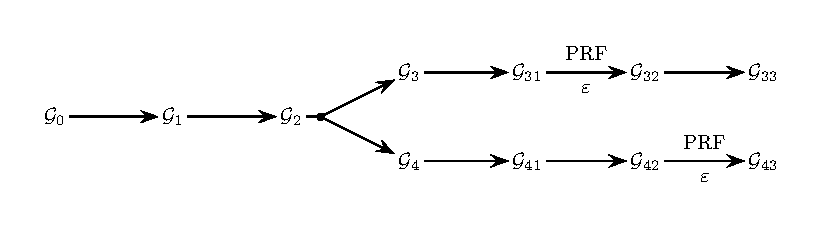
\includegraphics{figures/0803-proof-tree-i}
\end{center}
\caption{Game tree corresponding to the initial solution}
\label{fig:proof-tree-i}
\end{figure}

\paragraph{Initial solution.}
As $x \vee y = x \vee (\neg x \wedge y)$, then we can define two subgames:
\begin{align*}
\begin{game}{\GAME_3}
 &k \getsu \KSPACE\\
 &r_1, r_2 \getsu\RSPACE\\
 &\hat{r}_1 \gets \AD(r_1)\\
 &t_1 \gets f(\ID_1\|\ID_2\|\hat{r}_1\|r_2,k)\\
 &\hat{r}_2, \hat{t}_1 \gets \AD(r_2, t_1)\\
 &\IF f(\ID_1\|\ID_2\|r_1\|\hat{r}_2,k) \neq \hat{t}_1 \enspace\THEN \RETURN 0\\
 &t_2 \gets f(\ID_1\|\hat{r}_2,k)\\
 &\hat{t}_2 \gets \AD(t_2)\\
 &\IF f(\ID_1\|r_2,k) \neq \hat{t}_2 \enspace \RETURN 0\\
 &\RETURN [r_1\neq \hat{r}_1]  \enspace
\end{game}
&&
\begin{game}{\GAME_4}
 &k \getsu \KSPACE\\
 &r_1, r_2 \getsu\RSPACE\\
 &\hat{r}_1 \gets \AD(r_1)\\
 &t_1 \gets f(\ID_1\|\ID_2\|\hat{r}_1\|r_2,k)\\
 &\hat{r}_2, \hat{t}_1 \gets \AD(r_2, t_1)\\
 &\IF f(\ID_1\|\ID_2\|r_1\|\hat{r}_2,k) \neq \hat{t}_1 \enspace\THEN \RETURN 0\\
 &t_2 \gets f(\ID_1\|\hat{r}_2,k)\\
 &\hat{t}_2 \gets \AD(t_2)\\
 &\IF f(\ID_1\|r_2,k) \neq \hat{t}_2 \enspace \RETURN 0\\
 &\RETURN [r_1 \iseq \hat{r}_1] \wedge [r_2\neq \hat{r}_2] \enspace
\end{game}
\end{align*}
such that
\begin{align*}
\pr{\GAME_2^\AD = 1} \leq \pr{\GAME_3^\AD = 1} + \pr{\GAME_4^\AD = 1}\enspace.
\end{align*}
Next, we will  bound the success probability of an adversary against these two games. For the game $\GAME_3$, we can upperbound the success probability of an adversary by converting $\GAME_3$ into an easier game
\begin{align*}
\begin{game}{\GAME_{31}}
 &k \getsu \KSPACE\\
 &r_1, r_2 \getsu\RSPACE\\
 &\hat{r}_1 \gets \AD(r_1)\\
 &t_1 \gets f(\ID_1\|\ID_2\|\hat{r}_1\|r_2,k)\\
 &\hat{r}_2, \hat{t}_1 \gets \AD(r_2, t_1)\\
 &\IF f(\ID_1\|\ID_2\|r_1\|\hat{r}_2,k) \neq \hat{t}_1 \enspace\THEN \RETURN 0\\
 &\RETURN [r_1\neq \hat{r_1}]  \enspace.
\end{game}
\end{align*}

Moreover, as $f$ is a $(t,\varepsilon)$-pseudorandom function, there is at most $\varepsilon$ distance between the games $\GAME_{31}$ and the game 
\begin{align*}
\begin{game}{\GAME_{32}}
 &f\gets\FALL\\
 &r_1, r_2 \getsu\RSPACE\\
 &\hat{r}_1 \gets \AD(r_1)\\
 &t_1 \gets f(\ID_1\|\ID_2\|\hat{r}_1\|r_2)\\
 &\hat{r}_2, \hat{t}_1 \gets \AD(r_2, t_1)\\
 &\IF f(\ID_1\|\ID_2\|r_1\|\hat{r}_2) \neq \hat{t}_1 \enspace\THEN \RETURN 0\\
 &\RETURN [r_1\neq \hat{r}_1]  \enspace.
\end{game}
\end{align*}
in which the function is changed into a random function. Note that adversary $\AD$ can win only if it outputs $\hat{r}_1\neq r_1$. We can easily modify $\AD$ to always output $\hat{r}_1\neq r_1$ by increasing the running time by a small constant. This change can only increase the success probability. Thus, we can further only observe adversaries $\AD$  that always output $\hat{r}_1\neq r_1$. If $\hat{r}_1\neq r_1$ then also $\ID_1\|\ID_2\|\hat{r_1}\|r_2 \neq \ID_1\|\ID_2\|r_1\|\hat{r_2}$ and thus the random function $f$ is evaluated at two different arguments. Consequently, we can replace function calls by random sampling. This leads to the following game:
\begin{align*}
\begin{game}{\GAME_{33}}
 &r_1, r_2 \getsu\RSPACE\\
 &\hat{r}_1 \gets \AD(r_1)\\
 &t_1 \getsu\TTT\\
 &\hat{r}_2, \hat{t}_1 \gets \AD(r_2, t_1)\\
 &\dhat{t}_1\getsu\TTT\\
 &\IF \dhat{t}_1 \neq \hat{t}_1 \enspace\THEN \RETURN 0\\
 &\RETURN [r_1\neq \hat{r}_1]  \enspace.
\end{game}
\end{align*}
As the adversary chooses $\hat{t}_1$ before $\dhat{t}_1$ is sampled, we get
\begin{align*}
\pr{\GAME_{33}^\AD=1}=\frac{1}{\abs{T}}\enspace,
\end{align*}
which itself implies 
\begin{align*}
\pr{\GAME_3^\AD=1}\leq\pr{\GAME_{31}^\AD=1}\leq \pr{\GAME_{32}^\AD=1}+\varepsilon\leq\pr{\GAME_{23}^\AD=1}+\varepsilon\leq \frac{1}{\abs{T}}+\varepsilon\enspace.
\end{align*}

Now consider the game $\GAME_4$. In this game $\AD$ must create $r_1 = \hat{r}_1$ to win and thus we can always modify the adversary to output $r_1 = \hat{r}_1$ without decreasing the success probability. However, then the first interaction $\hat{r}_1\gets\AD(r_1)$ is unnecessary. Therefore, we can further simplify the security game as follows:
\begin{align*}
\begin{game}{\GAME_{41}}
 &k \getsu \KSPACE\\
 &r_1, r_2 \getsu\RSPACE\\
 &t_1 \gets f(\ID_1\|\ID_2\|r_1\|r_2,k)\\
 &\hat{r}_2, \hat{t}_1 \gets \AD(r_2, t_1)\\
 &\IF f(\ID_1\|\ID_2\|r_1\|\hat{r}_2,k) \neq \hat{t}_1 \enspace \RETURN 0\\
 &t_2 \gets f(\ID_1\|\hat{r}_2,k)\\
 &\hat{t}_2 \gets \AD(t_2)\\
 &\IF f(\ID_1\|r_2,k) \neq \hat{t}_2 \enspace \RETURN 0\\
 &\RETURN [r_2\neq \hat{r}_2] \enspace.
\end{game}
\end{align*}
To simplify the analysis, we can relax the game $\GAME_{41}$ by dropping the first check:
\begin{align*}
\begin{game}{\GAME_{42}}
 &k \getsu \KSPACE\\
 &r_1, r_2 \getsu\RSPACE\\
 &t_1 \gets f(\ID_1\|\ID_2\|r_1\|r_2,k)\\
 &\hat{r}_2, \hat{t}_1 \gets \AD(r_2, t_1)\\
 &t_2 \gets f(\ID_1\|\hat{r}_2,k)\\
 &\hat{t}_2 \gets \AD(t_2)\\
 &\IF f(\ID_1\|r_2,k) \neq \hat{t}_2 \enspace \RETURN 0\\
 &\RETURN [r_2\neq \hat{r}_2] \enspace.
\end{game}
\end{align*}
Again, this can only increase the success probability. The game $\GAME_{42}$ has distance at most $\varepsilon$  from the game where $f$  is replaced by a random function. Again the adversary $\AD$ must output $r_2\neq \hat{r}_2$ to succeed and by using the analogous reasoning as above we can consider only such  adversaries $\AD$ that always output $r_2\neq \hat{r}_2$. Again, if $r_2\neq \hat{r}_2$ then also $\ID_1\|r_2\neq \ID_1\| \hat{r_2}$. Since the third function argument $\ID_1\|\ID_2\|r_1\|r_2$ has different length than the others, the random function $f$ is evaluated on distinct inputs and we can replace function calls by random sampling without changing the semantics of the game. This leads to the following game:
\begin{align*}
\begin{game}{\GAME_{43}}
 &k \getsu \KSPACE\\
 &r_1, r_2 \getsu\RSPACE\\
 &t_1 \getsu\TTT\\
 &\hat{r}_2, \hat{t}_1 \gets \AD(r_2, t_1)\\
 &t_2 \getsu \TTT\\
 &\hat{t}_2 \gets \AD(t_2)\\
 &\dhat{t}_2 \getsu\TTT\\
 &\IF \dhat{t}_2 \neq \hat{t}_2 \enspace \RETURN 0\\
 &\RETURN [r_2\neq \hat{r}_2] \enspace.
\end{game}
\end{align*}
As before, we see that in $\GAME_{43}$, the adversary chooses $\hat{t}_2$ before $\dhat{t}_2$ is sampled and thus we can establish
\begin{align*}
\pr{\GAME_4^\AD=1}\leq\pr{\GAME_{41}^\AD=1}\leq \pr{\GAME_{42}^\AD=1}+\varepsilon\leq\pr{\GAME_{43}^\AD=1}+\varepsilon\leq \frac{1}{\abs{T}}+\varepsilon\enspace.
\end{align*}
Now by combining the results, we obtain a reasonable but loose bound  
\begin{align*}
\ADVWIN{\GAME_0}{\AD} \leq \Pr{[\GAME_2^\AD = 1]} \leq \Pr{[\GAME_3^\AD = 1]} + \Pr{[\GAME_4^\AD = 1]} \leq \frac{2}{\abs{\TSPACE}} + 2 \varepsilon\enspace.
\end{align*}

\begin{figure}[t]
\begin{center}
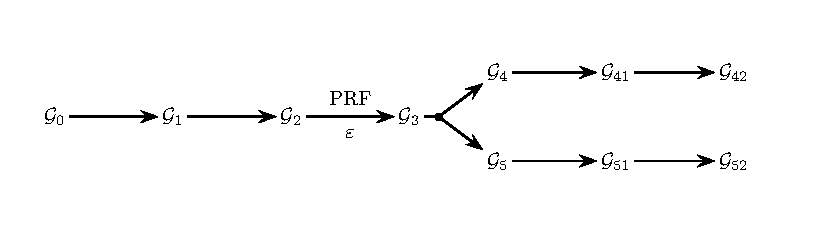
\includegraphics{figures/0803-proof-tree-ii}
\end{center}
\caption{Game tree corresponding to the first improvement}
\label{fig:proof-tree-ii}
\end{figure}

\paragraph{First improvement.}
The first solution is sub-optimal, as we had to replace function $f$ with a random function in both branches of the proof. We could do it directly by defining the game 
\begin{align*}
  \begin{game}{\GAME_3}
	& f \getsu \FFFALL \\
	& r_1 \getsu \RSPACE \\
	& \hat{r}_1 \gets \AD(r_1) \\
	& r_2 \getsu \RSPACE \\
	& t_1 \gets f(\ID_1 || \ID_2 || \hat{r}_1 || r_2) \\
	& \hat{r}_2, \hat{t}_1 \gets \AD(r_2, t_1) \\
	& \IF f(\ID_1 || \ID_2 || r_1 || \hat{r}_2) \neq \hat{t}_1 \ \THEN \RETURN 0 \\
	& t_2 \gets f(\ID_1 || \hat{r}_2) \\
	& \hat{t}_2 \gets \AD(t_2) \\
	& \IF f(\ID_1 || r_2) \neq \hat{t}_2 \ \THEN \RETURN 0 \\
	& \RETURN [r_1 \neq \hat{r}_1] \vee [r_2 \neq \hat{r}_2]
  \end{game}
\end{align*}
Since $f$ is a $(t,\varepsilon)$-pseudorandom function and the key $k$ is not leaked to the adversary, the change in the success probability is bounded:
\begin{align*}
\abs{\pr{\GAME_2^\AD=1}-\pr{\GAME_3^\AD=1}}\leq\varepsilon\enspace.
\end{align*}
Now for any $\AD$, we can decompose the success probability into a sum
\begin{align*}
 \pr{\GAME_3^\AD = 1} & = \pr{\GAME_3^\AD = 1 \wedge r_1 \neq \hat{r}_1} + 
 \pr{\GAME_3^\AD = 1 \land r_1 = \hat{r}_1 \land r_2 \neq \hat{r}_2}\enspace. 
\end{align*}
For both terms on the right, we can define corresponding games:
\begin{align*}
  \begin{game}{\GAME_4}
	& f \getsu \FFFALL \\
	& r_1 \getsu \RSPACE \\
	& \hat{r}_1 \gets \AD(r_1) \\
	& r_2 \getsu \RSPACE \\
	& t_1 \gets f(\ID_1 || \ID_2 || \hat{r}_1 || r_2) \\
	& \hat{r}_2, \hat{t}_1 \gets \AD(r_2, t_1) \\
	& \IF f(\ID_1 || \ID_2 || r_1 || \hat{r}_2) \neq \hat{t}_1 \ \THEN \RETURN 0 \\
	& t_2 \gets f(\ID_1 || \hat{r}_2) \\
	& \hat{t}_2 \gets \AD(t_2) \\
	& \IF f(\ID_1 || r_2) \neq \hat{t}_2 \ \THEN \RETURN 0 \\
	& \RETURN [r_1 \neq \hat{r}_1] 
  \end{game}\qquad\qquad
  \begin{game}{\GAME_5}
	& f \getsu \FFFALL \\
	& r_1 \getsu \RSPACE \\
	& \hat{r}_1 \gets \AD(r_1) \\
	& r_2 \getsu \RSPACE \\
	& t_1 \gets f(\ID_1 || \ID_2 || \hat{r}_1 || r_2) \\
	& \hat{r}_2, \hat{t}_1 \gets \AD(r_2, t_1) \\
	& \IF f(\ID_1 || \ID_2 || r_1 || \hat{r}_2) \neq \hat{t}_1 \ \THEN \RETURN 0 \\
	& t_2 \gets f(\ID_1 || \hat{r}_2) \\
	& \hat{t}_2 \gets \AD(t_2) \\
	& \IF f(\ID_1 || r_2) \neq \hat{t}_2 \ \THEN \RETURN 0 \\
	& \RETURN \smash{[r_1 \iseq \hat{r}_1]} \wedge [r_2 \neq \hat{r}_2]\enspace.
  \end{game}
\end{align*}
Note that in the game $\GAME_4$ it is straightforward to pass the second check by submitting $\hat{r}_2=r_2$ and $\hat{t}_2=t_2$. Thus the second check does not make the game harder for the adversary and we can drop it.  As  a result, we obtain the following game:
\begin{align*}
  \begin{game}{\GAME_{41}}
	& f \getsu \FFFALL \\
	& r_1 \getsu \RSPACE \\
	& \hat{r}_1 \gets \AD(r_1) \\
	& r_2 \getsu \RSPACE \\
	& t_1 \gets f(\ID_1 || \ID_2 || \hat{r}_1 || r_2) \\
	& \hat{r}_2, \hat{t}_1 \gets \AD(r_2, t_1) \\
	& \IF f(\ID_1 || \ID_2 || r_1 || \hat{r}_2) \neq \hat{t}_1 \ \THEN \RETURN 0 \\
	& \RETURN [r_1 \neq \hat{r}_1] 
  \end{game}
\end{align*}
The adversary can win this game only if $r_1 \neq \hat{r}_1$ and thus we can assume without loss of generality that $\AD$ always outputs $\hat{r}_1 \neq r_1$. As result, the function $f$ is evaluated on distinct arguments and both evaluations can be replaced with random sampling:
\begin{align*}
  \begin{game}{\GAME_{42}}
	& f \getsu \FFFALL \\
	& r_1 \getsu \RSPACE \\
	& \hat{r}_1 \gets \AD(r_1) \\
	& r_2 \getsu \RSPACE \\
	& t_1 \getsu \TTT\\
	& \hat{r}_2, \hat{t}_1 \gets \AD(r_2, t_1) \\
	& \dhat{t}_1\getsu\TTT\\
	& \IF \dhat{t}_1 \neq \hat{t}_1 \ \THEN \RETURN 0 \\
	& \RETURN [r_1 \neq \hat{r}_1] \enspace
  \end{game}
\end{align*}
which itself implies 
\begin{align*}
\pr{\GAME_{41}^\AD=1}=\frac{1}{\abs{\TTT}}\enspace.
\end{align*}
To analyse the game $\GAME_5$, note that for the analogous reasoning we can assume that  $\AD$ always outputs $\hat{r}_1=r_1$ and $\hat{r}_2\neq r_2$. As a result, we can simplify the game: 
\begin{align*}
  \begin{game}{\GAME_{51}}
	& f \getsu \FFFALL \\
	& r_1 \getsu \RSPACE \\
	& r_2 \getsu \RSPACE \\
	& t_1 \gets f(\ID_1 || \ID_2 || r_1 || r_2) \\
	& \hat{r}_2, \hat{t}_1 \gets \AD(r_2, t_1) \\
	& \IF f(\ID_1 || \ID_2 || r_1 || \hat{r}_2) \neq \hat{t}_1 \ \THEN \RETURN 0 \\
	& t_2 \gets f(\ID_1 || \hat{r}_2) \\
	& \hat{t}_2 \gets \AD(t_2) \\
	& \IF f(\ID_1 || r_2) \neq \hat{t}_2 \ \THEN \RETURN 0 \\
	& \RETURN \smash{[r_1 \iseq \hat{r}_1]} \wedge [r_2 \neq \hat{r}_2]\enspace.
  \end{game}
\end{align*}
Again, it is easy to see that under these assumption all four evaluations of $f$ are done on distinct inputs and we can replace them all with random sampling:
\begin{align*}
  \begin{game}{\GAME_{52}}
	& r_1 \getsu \RSPACE \\
	& r_2 \getsu \RSPACE \\
	& t_1 \getsu \TTT \\
	& \hat{r}_2, \hat{t}_1 \gets \AD(r_2, t_1) \\
	& \dhat{t}_1\getsu\TTT\\
	& \IF  \dhat{t}_1 \neq \hat{t}_1 \ \THEN \RETURN 0 \\
	& t_2 \gets f(\ID_1 || \hat{r}_2) \\
	& \hat{t}_2 \gets \AD(t_2) \\
	& \dhat{t}_2\getsu\TTT\\
	& \IF \dhat{t}_2 \neq \hat{t}_2 \ \THEN \RETURN 0 \\
	& \RETURN \smash{[r_1 \iseq \hat{r}_1]} \wedge [r_2 \neq \hat{r}_2]\enspace.
  \end{game}
\end{align*}
It is straightforward to see that the adversary passes the first check with the probability   $\frac{1}{\abs{\TTT}}$ and both checks with the probability
\begin{align*}
\pr{\GAME_{52}^\AD=1}=\frac{1}{\abs{\TTT}^2}\enspace.
\end{align*}
By combining all results, we get a much tighter bound:
\begin{align*}
\pr{\GAME_0^\AD=1}\leq \pr{\GAME_3^\AD=1}+\varepsilon\leq \pr{\GAME_{42}^\AD=1}+\pr{\GAME_{52}^\AD=1}+\varepsilon\leq \frac{1}{\abs{\TTT}}+\frac{1}{\abs{\TTT}^2}+\varepsilon\enspace.
\end{align*} 

\begin{figure}[t]
\begin{center}
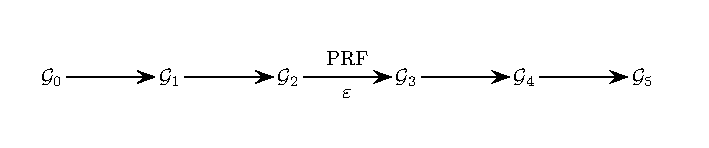
\includegraphics{figures/0803-proof-tree-iii}
\end{center}
\caption{Game tree corresponding to the final proof}
\label{fig:proof-tree-iii}
\end{figure}


\paragraph{Final proof.}
The result obtained in the last proof is much better but still sub-optimal. Intuitively, the adversary must guess either the value of $f(\ID_1 || \ID_2 || r_1 || \hat{r}_2)$ or
$f(\ID_1 || r_2)$ in game $\GAME_3$ depending whether it outputs $\hat{r}_1\neq r_1$ or $\hat{r}_2\neq r_2$. Thus, we should be able to prove $\ADVWIN{\GAME_3}{\AD}\leq\frac{1}{\abs{\TTT}}$, although we somehow obtained the slightly looser bound:
\begin{align*}
\pr{\GAME_3^\AD=1}\leq \frac{1}{\abs{\TTT}}+\frac{1}{\abs{\TTT}^2} \enspace.
\end{align*}
The reason why the bound is sub-optimal is subtle. First of all note that the claim
\begin{align*}
\pr{\GAME_3^\AD=1}= \pr{\GAME_4^\AD=1}+ \pr{\GAME_5^\AD=1} 
\end{align*}
is tight. Also, the bounds 
\begin{align*}
\pr{\GAME_4^\AD=1}&\leq \pr{\GAME_{41}^\AD=1}\\ 
\pr{\GAME_5^\AD=1}&\leq \pr{\GAME_{51}^\AD=1} 
\end{align*}
are separately taken optimal. However, we maximise probabilities in both branches separately and this leads to sub-optimality:
\begin{align*}
\max_\AD\pr{\GAME_3^\AD=1} < \max_\AD\pr{\GAME_4^\AD=1}+ \max_\AD\pr{\GAME_5^\AD=1}\enspace.
\end{align*}  
To getter better result, we have to rewrite the game $\GAME_3$ in a more revealing way:
\begin{align*}
  \begin{game}{\GAME_4}
	& f \getsu \FFFALL \\
	& r_1 \getsu \RSPACE \\
	& \hat{r}_1 \gets \AD(r_1) \\
	& r_2 \getsu \RSPACE \\
	& t_1 \gets f(\ID_1 || \ID_2 || \hat{r}_1 || r_2) \\
	& \hat{r}_2, \hat{t}_1 \gets \AD(r_2, t_1) \\
	& \IF r_1\neq \hat{r}_1\ \THEN\\
	& \begin{cblock}
	   &\IF f(\ID_1 || \ID_2 || r_1 || \hat{r}_2) \neq \hat{t}_1\ \THEN \RETURN 0\\
	   & t_2 \gets f(\ID_1 || \hat{r}_2) \\
	   & \hat{t}_2 \gets \AD(t_2) \\
	   & \IF f(\ID_1 || r_2) \neq \hat{t}_2 \ \THEN \RETURN 0 \\
	   & \RETURN 1
	& \end{cblock}\\ 
	& \ELSE \IF r_2\neq \hat{r}_2\ \THEN\\
	& \begin{cblock}   
	   & t_2 \gets f(\ID_1 || \hat{r}_2) \\
	   & \hat{t}_2 \gets \AD(t_2) \\
	   & \IF f(\ID_1 || r_2) \neq \hat{t}_2 \ \THEN \RETURN 0 \\
	   & \RETURN 1
	  \end{cblock}\\   
	& \ELSE \RETURN 0\enspace.
  \end{game}
\end{align*}
It is easy to see that the adversary can win the branch $r_1\neq \hat{r}_1$ if it manages to pass the first test by choosing $\hat{r}_2=r_2$ and $\hat{t}_2=t_2$. Hence, we can drop the second test. As $r_1\neq \hat{r}_1$ in this branch, we can conclude that $\ID_1 || \ID_2 || r_1 || \hat{r}_2\neq \ID_1 || \ID_2 || \hat{r}_1 || r_2$ and thus we can replace the evaluation of $f(\ID_1 || \ID_2 || r_1 || \hat{r}_2)$ by random sampling. In the branch 
$r_2\neq \hat{r}_2$, we query the function $f$ on an argument that has different length than the previous argument $\ID_1 || \ID_2 || \hat{r}_1 || r_2$. Hence, we can replace this function evaluation also with the random sampling. This leads to a modified game:
\begin{align*}
  \begin{game}{\GAME_5}
	& f \getsu \FFFALL \\
	& r_1 \getsu \RSPACE \\
	& \hat{r}_1 \gets \AD(r_1) \\
	& r_2 \getsu \RSPACE \\
	& t_1 \gets f(\ID_1 || \ID_2 || \hat{r}_1 || r_2) \\
	& \hat{r}_2, \hat{t}_1 \gets \AD(r_2, t_1) \\
	& \IF r_1\neq \hat{r}_1\ \THEN\\
	& \begin{cblock}
	   & \dhat{t}_1\getsu\TTT\\
	   &\IF \dhat{t}_1 \neq \hat{t}_1\ \THEN \RETURN 0\\
	   & \RETURN 1
	& \end{cblock}\\ 
	& \ELSE \IF r_2\neq \hat{r}_2\ \THEN\\
	& \begin{cblock}   
	   & t_2 \gets f(\ID_1 || \hat{r}_2) \\
	   & \hat{t}_2 \gets \AD(t_2) \\
	   & \dhat{t}_2\getsu\TTT\\
	   & \IF \dhat{t}_2 \neq \hat{t}_2 \ \THEN \RETURN 0 \\
	   & \RETURN 1
	  \end{cblock}\\   
	& \ELSE \RETURN 0\enspace.
  \end{game}
\end{align*}
From this construction it is evident that 
\begin{align*}
\pr{\GAME_5^\AD=1}=\pr{r_1\neq\hat{r}_1}\cdot\pr{\smash{\dhat{t}_1=\hat{t}_1}}+\pr{r_1=\hat{r}_1\wedge r_2\neq\hat{r}_2}\cdot\pr{\smash{\dhat{t}_2=\hat{t}_2}}\leq\frac{1}{\abs{\TTT}}\enspace
\end{align*}
which gives the optimal success bound
\begin{align*}
\pr{\GAME_0^\AD=1}\leq \pr{\GAME_3^\AD=1}+\varepsilon\leq \pr{\GAME_{5}^\AD=1}+\varepsilon\leq \frac{1}{\abs{\TTT}}+\varepsilon\enspace.
\end{align*}

\paragraph{Conclusion.}
The example proofs show that splitting the proof into several branches is a powerful technique. However, there is a cost to pay. First of all, you have to use cryptographic assumptions separately in each branch and this leads to more relaxed upper bounds compared to the case when you use cryptographic assumptions before branching. Secondly, even the game simplification through branching can lead to sub-optimal result. The latter does not mean you should avoid branching.  Branching is a valuable technique, as it provides a fast way to get the initial bound that can be later reduced by more advanced analysis.       
 
       
\end{solution}
\end{document}